\documentclass[10pt]{article}
\usepackage[left=1.5cm,right=1.5cm,top=1.5cm,bottom=1.5cm,landscape]{geometry}
\usepackage{booktabs}
\usepackage{longtable}
\usepackage{array}
\usepackage[table]{xcolor}
\usepackage{hyperref}
\usepackage{enumitem}
\usepackage{tikz}
\usetikzlibrary{shapes.arrows,positioning,arrows.meta,fit,backgrounds}
\usepackage{fancyhdr}

\definecolor{inputred}{RGB}{180,0,0}
\definecolor{outputblue}{RGB}{0,0,180}
\definecolor{awsorange}{RGB}{255,153,0}
\definecolor{sectionblue}{RGB}{31,86,115}
\definecolor{panelblue}{RGB}{31,86,115}
\definecolor{tabA}{RGB}{66,133,244}
\definecolor{tabB}{RGB}{255,152,0}
\definecolor{tabC}{RGB}{52,168,83}
\definecolor{tabD}{RGB}{154,205,50}
\definecolor{tabE}{RGB}{156,39,176}
\definecolor{normgray}{RGB}{100,100,100}

\pagestyle{fancy}
\fancyhf{}
\fancyfoot[C]{\thepage}
\fancyhead[L]{\small TechBrazil / PROPAG Data Inventory --- v2 (Fev 2026)}
\fancyhead[R]{\small \today}
\renewcommand{\headrulewidth}{0.4pt}

\title{\textbf{TechBrazil / PROPAG Data Inventory}\\[0.3em]\large Ferramenta de Apoio Analítico --- Plano de Aplicação\\[0.3em]\normalsize Inventário de Dados por Aba do Aplicativo Shiny\\[0.2em]\small Versão 2 --- Fevereiro 2026}
\author{Suhas Parandekar}
\date{\today}

\begin{document}
\maketitle
\thispagestyle{fancy}

\section*{Aplicativo Principal: BM\_FGV\_Propag2.R}

Aplicativo Shiny com 15 abas organizadas por código de cores temático:

\begin{tabular}{lll}
\textcolor{tabA}{$\blacksquare$} \textbf{Azul} & A1--A2 & Demografia \\
\textcolor{tabB}{$\blacksquare$} \textbf{Laranja} & B1--B3 & Finanças PROPAG \\
\textcolor{tabC}{$\blacksquare$} \textbf{Verde} & C1--C4 & Oferta EPT \\
\textcolor{tabD}{$\blacksquare$} \textbf{Verde-Lima} & D1--D3 & Demanda EPT \\
\textcolor{tabE}{$\blacksquare$} \textbf{Roxo} & E1--E2 & Conexão Oferta-Demanda \\
\end{tabular}

\vspace{0.5em}
\noindent\textbf{Bucket S3:} \texttt{techbrazildata} (us-east-1) | \textbf{Estrutura:} \texttt{rawdata/} (dados brutos) $\rightarrow$ \texttt{working/} (dados processados)

\vspace{0.5em}
\noindent\textbf{Marco Normativo (atualizado Fev 2026):}

\begin{tabular}{lp{18cm}}
\textcolor{normgray}{$\bullet$} & Lei Complementar nº 212/2025 (13 Jan) --- Institui o PROPAG \\
\textcolor{normgray}{$\bullet$} & Decreto nº 12.433/2025 (14 Abr) --- Regulamenta LC 212, institui Juros por Educação (Arts.\ 68--77) \\
\textcolor{normgray}{$\bullet$} & Portaria MF nº 2.899/2025 (27 Nov) --- Adesão, dívidas, ativos, FEF, prestação de contas, encargos \\
\textcolor{normgray}{$\bullet$} & Portaria MF nº 3.066/2025 (11 Dez) --- Complementa operacionalização FEF e prazos \\
\textcolor{normgray}{$\bullet$} & Portaria MEC nº 930/2025 (30 Dez) --- Regulamenta Juros por Educação: metas, ofertas EPTNM, PNEPT \\
\textcolor{normgray}{$\bullet$} & Portaria STN/MF nº 369/2026 (11 Fev) --- Aprova modelo demonstrativo comprovação de aplicação de recursos \\
\end{tabular}

\vspace{1em}
\hrule
\vspace{0.8em}

%==============================================================================
% PANEL A1
%==============================================================================
\subsection*{\textcolor{tabA}{$\blacksquare$} Aba A1: Transição Demográfica --- Projeções Populacionais por Faixa Etária}

\noindent\textbf{Descrição:} Análise das mudanças no perfil etário da população brasileira (2000--2070) por região e estado, identificando pontos de transição demográfica (crossover 0-14 vs 60+).

\begin{center}
\small
\begin{tabular}{p{3.5cm}p{4.5cm}p{5cm}p{9cm}}
\toprule
\textbf{Objeto Shiny} & \textbf{Script Fonte} & \textbf{Dados Brutos (S3)} & \textbf{Variáveis Principais} \\
\midrule
\texttt{pop01\_70b} & \texttt{prelims/população/} \newline \texttt{br\_pop1a.R} & \texttt{rawdata/ibge/} \newline \texttt{projecoes\_2024\_tab3\_} \newline \texttt{grupos\_etarios\_especificos.xlsx} & ANO, SIGLA, LOCAL, POP\_T, 0-14\_T, 15-17\_T, 18-21\_T, 15-59\_T, 60+\_T, P\_* (proporções), Crossover\_Flag/Value \\
\bottomrule
\end{tabular}
\end{center}

\noindent\textbf{Agregações Criadas:} Amazônia Legal (9 UFs), Nordeste\_r (8 UFs excl.\ MA), Centro-Oeste\_r (3 UFs excl.\ MT)

\vspace{0.8em}
\hrule
\vspace{0.8em}

%==============================================================================
% PANEL A2
%==============================================================================
\subsection*{\textcolor{tabA}{$\blacksquare$} Aba A2: EPT e População --- População 15-19 anos e Matrículas EPT/Ensino Médio}

\noindent\textbf{Descrição:} Comparação entre população de 15-19 anos e matrículas na EPT/Ensino Médio, com acompanhamento das metas do PNE Meta 11.

\begin{center}
\small
\begin{tabular}{p{3.5cm}p{4.5cm}p{5cm}p{9cm}}
\toprule
\textbf{Objeto Shiny} & \textbf{Script Fonte} & \textbf{Dados Brutos (S3)} & \textbf{Variáveis Principais} \\
\midrule
\texttt{pop01\_70b} & (mesmo que A1) & (mesmo que A1) & 15-17\_T, 18-21\_T $\rightarrow$ cálculo 15-19\_T \\
\texttt{meta11a\_opcoes} & \texttt{prelims/mec/} \newline \texttt{censo\_garabed\_01a.R} & \texttt{working/mec\_inep/} \newline \texttt{df\_censo\_UF.rda} \newline \texttt{Tecnico\_FormaR\_Garabed1.rda} & ANO, SG\_UF, NM\_UF, QT\_MAT\_PROF\_TEC\_PROPAG, QT\_MAT\_MED, Meta11a\_opcao1/2/3 \\
\texttt{df\_codes\_ibge} & \texttt{prelims/mapas/} \newline \texttt{codes\_ibge.R} & \texttt{working/ibge/} \newline \texttt{df\_pibmunis.rda} & CO\_5RGRANDE, NM\_5RGRANDE, CO\_UF, SG\_UF, NM\_UF, CO\_MUN, NM\_MUN, CO\_RGIMED, CO\_RGINTM \\
\bottomrule
\end{tabular}
\end{center}

\noindent\textbf{Derivações no Shiny:} \texttt{ept\_combined\_data} (join pop + enrollment), \texttt{PCT\_MAT\_EPT}, \texttt{PCT\_MAT\_MED}, \texttt{ept\_meta11\_df} (meta = 3x 2013)

\vspace{0.8em}
\hrule
\vspace{0.8em}

%==============================================================================
% PANELS B1-B3
%==============================================================================
\subsection*{\textcolor{tabB}{$\blacksquare$} Abas B1--B3: Financiamento PROPAG --- Simulações e Cenários}

\noindent\textbf{Descrição:} Simulação do impacto financeiro do PROPAG com diferentes cenários de adesão, abatimento, FEF e investimento em EPT. \textit{Nota: Período de adesão encerrado em 31/12/2025 (Portaria MF 2.899, Art.\ 2). Abas mantidas para compreensão dos cenários escolhidos pelos estados.}

\begin{center}
\small
\begin{tabular}{p{3.5cm}p{4.5cm}p{5cm}p{9cm}}
\toprule
\textbf{Objeto Shiny} & \textbf{Script Fonte} & \textbf{Dados Brutos} & \textbf{Variáveis Principais} \\
\midrule
\texttt{df\_2a, df\_2b, df\_2c} \newline \texttt{df\_3a, df\_3b, df\_3c} \newline \texttt{df\_4a, df\_4b, df\_nd} & \texttt{produtos\_avila\_vidal/} \newline \texttt{avila\_vidal01.R} & \texttt{rawdata/fgv/} \newline \texttt{fgv\_fin2b.xlsx} \newline (9 sheets, dados FGV/Vidal) & NM\_UF, DIVIDA, Distr\_FEF, Valor\_Abat, Saldo2025--2054, ApoFEF2025--2054, InvDir2025--2054, JurPag2025--2054 \\
\texttt{dfcen\_val} & \texttt{produtos\_avila\_vidal/} \newline \texttt{avila\_vidal01.R} & (gerado internamente) & A (abatimento), G (FEF), I (investimento), J (juros), valid, opcao \\
\texttt{propag\_ept\_financeiro} & (arquivo .rds externo) & Scraping portal PROPAG & UF, Estado, saldo\_mar25, amort\_extr, FEF\_*, EPT\_* \\
\bottomrule
\end{tabular}
\end{center}

\noindent\textbf{Cenários:} II-A/B/C (Juros 0\%), III-A/B/C (Juros 1\%), IV-A/B (Juros 2\%), ND (Não Adere, 4\%). Ref: Portaria STN/MF 369/2026 --- modelo demonstrativo para comprovação.

\vspace{0.8em}
\hrule
\vspace{0.8em}

%==============================================================================
% PANELS C1-C4
%==============================================================================
\subsection*{\textcolor{tabC}{$\blacksquare$} Abas C1--C4: Oferta EPT --- Projeção, Planificação, Redes e Modelo}

\noindent\textbf{Descrição:} Análise da oferta de EPT vs Meta 11, projeção de matrículas necessárias, e modelo econométrico de fatores determinantes. Ref: Portaria MEC 930/2025, Art.\ 3º--4º (metas PNE, patamar inicial Censo Escolar).

\begin{center}
\small
\begin{tabular}{p{3.5cm}p{4.5cm}p{5cm}p{9cm}}
\toprule
\textbf{Objeto Shiny} & \textbf{Script Fonte} & \textbf{Dados Brutos (S3)} & \textbf{Variáveis Principais} \\
\midrule
\texttt{meta11a\_opcoes} & (mesmo que A2) & (mesmo que A2) & Meta11a\_opcao1/2/3 para projeções \\
\texttt{df\_censo\_UF} & \texttt{prelims/mec/} \newline \texttt{matriculas1UF.R} & Microdados Censo Escolar \newline 2007--2024 & Agregações por UF, ano, dependência administrativa \\
\texttt{df\_pibmunis} & \texttt{prelims/municipios/} \newline \texttt{TB\_municipios1a.R} & \texttt{working/sqlite/} \newline \texttt{TB\_municipios.sqlite} & PIB por município 2002--2021 (43 variáveis) \\
\texttt{df\_residuals\_ols} & \texttt{prelims/modelo/} \newline \texttt{modelo\_ept3a.R} & Modelo OLS com efeitos fixos & Resíduos do modelo, fitted values, variáveis explicativas \\
\bottomrule
\end{tabular}
\end{center}

\vspace{0.8em}
\hrule
\vspace{0.8em}

%==============================================================================
% PANEL C3 DETAIL
%==============================================================================
\subsection*{\textcolor{tabC}{$\blacksquare$} Aba C3 Detalhe: Oferta EPT por Eixo e Curso}

\begin{center}
\small
\begin{tabular}{p{3.5cm}p{4.5cm}p{5cm}p{9cm}}
\toprule
\textbf{Objeto Shiny} & \textbf{Script Fonte} & \textbf{Dados Brutos (S3)} & \textbf{Variáveis Principais} \\
\midrule
\texttt{df\_censo\_supl\_tec23} \newline \texttt{df\_censo\_supl\_tec24} & \texttt{prelims/mec/} \newline \texttt{prepara\_censo\_escolar\_tecnico\_01a.R} & Microdados Censo Escolar \newline Suplemento Técnico & CO\_MUN, ANO, TP\_DEPENDENCIA, NO\_AREA\_CURSO, NO\_CURSO\_EDUC\_PROFISSIONAL, QT\_MAT\_CURSO\_TEC\_* \\
\texttt{df\_censo\_notin\_cnct} & \texttt{prelims/qbq/} \newline \texttt{qbq\_02a.R} & Cursos não mapeados no CNCT & Cursos do Censo sem correspondência CNCT \\
\bottomrule
\end{tabular}
\end{center}

\vspace{0.8em}
\hrule
\vspace{0.8em}

%==============================================================================
% PANELS D1-D3
%==============================================================================
\subsection*{\textcolor{tabD}{$\blacksquare$} Abas D1--D3: Demanda EPT --- Dinamismo Econômico, APLs e Informalidade}

\noindent\textbf{Descrição:} Análise da demanda por EPT baseada em dinamismo econômico municipal, arranjos produtivos locais (APLs) e formalidade do emprego. Suporta o requisito do Art.\ 71, §6º, III do Decreto 12.433 (justificativa de escolha de cursos).

\begin{center}
\small
\begin{tabular}{p{3.5cm}p{4.5cm}p{5cm}p{9cm}}
\toprule
\textbf{Objeto Shiny} & \textbf{Script Fonte} & \textbf{Dados Brutos (S3)} & \textbf{Variáveis Principais} \\
\midrule
\texttt{MUN\_dyna02\_21} & \texttt{prelims/municipios/} \newline \texttt{econ\_dynam1a.R} & \texttt{working/ibge/} \newline \texttt{df\_pibmunis.rda} & dynamism\_index, dynamism\_decile, period1/2\_avg\_growth \\
\texttt{qbq\_ocup\_cmento1} & \texttt{prelims/qbq/} \newline \texttt{qbq\_03a.R} & \texttt{working/qbq/} & cbo\_4dig, cbo\_familia, cbo\_gragru, ocupação normalizada \\
\texttt{cbo\_short\_names} & \texttt{prelims/qbq/} \newline \texttt{qbq\_03a.R} + \newline \texttt{cbo\_short\_names\_gemini.py} & \texttt{working/qbq/} \newline \texttt{cbo\_short\_names.rda} & cbo\_4dig, cbo\_familia, short\_name (nomes curtos 3--4 palavras via Gemini) \\
\texttt{df\_cbocod\_mun23} \newline \texttt{df\_cbocod\_mun24} & \texttt{prelims/rais/} \newline \texttt{rais\_apo4a.R} & RAIS vínculos municipais & Emprego formal por CBO e município \\
\bottomrule
\end{tabular}
\end{center}

\noindent\textbf{D1 --- Dinamismo:} Índice de dinamismo = média ponderada crescimento PIB pc (2002--2011 peso 1.0; 2012--2021 peso 1.5). Mapa e tabela com decis coloridos.

\noindent\textbf{D2 --- APLs:} Quociente Locacional (QL) identifica especialização. Prioridade: \textcolor{red}{Alta} (QL$\geq$5) | \textcolor{orange}{Média} (QL 2.5--5) | \textcolor{green!60!black}{Padrão} (QL 1.25--2.5). Tabela com pills coloridas. Modo correspondência APL-Cursos.

\noindent\textbf{D3 --- Informalidade:} Taxa de formalidade por município para ocupações EPT (RAIS + PNAD-C).

\vspace{0.8em}
\hrule
\vspace{0.8em}

%==============================================================================
% PANELS E1-E2
%==============================================================================
\subsection*{\textcolor{tabE}{$\blacksquare$} Abas E1--E2: Conexão Oferta-Demanda EPT e Escassez de Profissionais}

\noindent\textbf{Descrição:} Matching entre cursos EPT (CNCT) e ocupações (CBO) usando IA (embeddings semânticos + TF-IDF); diagnóstico de escassez de profissionais técnicos.

\begin{center}
\small
\begin{tabular}{p{3.5cm}p{4.5cm}p{5cm}p{9cm}}
\toprule
\textbf{Objeto Shiny} & \textbf{Script Fonte} & \textbf{Dados Brutos (S3)} & \textbf{Variáveis Principais} \\
\midrule
\texttt{df\_mat\_uf/eixo/area/curso} & \texttt{prelims/qbq/qbq\_02a.R} & Censo Escolar agregado & Matrículas por UF, Eixo, Área, Curso \\
\texttt{df\_exarcu} & \texttt{prelims/qbq/qbq\_02a.R} & Catálogo CNCT & IDX\_EIXCUR, Eixo, Área, Denominação do Curso \\
\texttt{rais\_cbo6\_uf23/24} & \texttt{prelims/rais/rais2a.R} & RAIS microdados & Emprego por CBO 6-dígitos e UF \\
\texttt{cnct\_qbq\_matches2} \newline \texttt{qbq\_cnct\_matches2} & \texttt{prelims/qbq/} \newline \texttt{qbq\_cnct\_06a.R} & Pipeline semântico \newline (10 scripts, ver seção) & Curso $\leftrightarrow$ Ocupação (score similaridade) \\
\texttt{caged\_rais\_cnct\_} \newline \texttt{2020\_2024\_shiny} & \texttt{prelims/caged/} \newline \texttt{2\_preprocess\_caged\_} \newline \texttt{rais\_shiny.R} & CAGED + RAIS 2020--2024 & Fluxos admissão/desligamento, salários, rotatividade por curso \\
\bottomrule
\end{tabular}
\end{center}

\noindent\textbf{Indicadores de Escassez (E2):} dif\_sal\_adm\_des\_pc (gap salarial), tx\_rotatividade, estoque\_liquido, tipologia\_escassez

\vspace{1em}
\hrule
\vspace{1em}

%==============================================================================
% QBQ-CNCT MATCHING PIPELINE
%==============================================================================
\subsection*{Pipeline de Matching Semântico CNCT-CBO (11 scripts)}

\noindent Matching entre 218 cursos CNCT e 1.899 ocupações QBQ usando embeddings multilíngues (intfloat/multilingual-e5-large) + Pinecone + TF-IDF. Saídas pré-computadas no S3 --- \textbf{não necessário re-executar}.

\begin{center}
\small
\begin{tabular}{p{1.5cm}p{4cm}p{4.5cm}p{12cm}}
\toprule
\textbf{Etapa} & \textbf{Script} & \textbf{Saída} & \textbf{Função} \\
\midrule
1 & \texttt{cnct1a.py} & df\_cnct2025a.pkl/.csv & Processar catálogo CNCT, criar códigos IDX\_EIXARECUR \\
1 & \texttt{qbq\_04a.R} & df\_cnct\_cbo.rda, df\_cnct2025b.pkl & Extrair CBOs do CNCT, expandir 4-dígitos, criar blobs texto \\
1 & \texttt{qbq\_cnct1b.py} & df\_censo\_cbo\_matched.pkl & Alinhar CBOs dos cursos CNCT com ocupações QBQ \\
2 & \texttt{qbq\_cnct2a.py} & Índice Pinecone & Gerar embeddings e popular banco vetorial \\
3 & \texttt{qbq\_cnct3a.py} & tfidf\_vectors\_*.pkl & Calcular vetores TF-IDF baseline \\
4 & \texttt{qbq\_cnct4b.R} & *\_blob.pkl, tfidf\_vectors\_cnct.pkl & Concatenar campos CNCT em blobs de texto, calcular TF-IDF \\
5 & \texttt{qbq\_cnct5a.py} & Pinecone (upsert) & Upload blobs ao Pinecone \\
5 & \texttt{qbq\_cnct5b.py} & cnct\_qbq\_matches.csv & Matching Curso $\rightarrow$ Ocupação (top 50) \\
5 & \texttt{qbq\_cnct5c.py} & qbq\_cnct\_matches.csv & Matching Ocupação $\rightarrow$ Curso (top 20) \\
5 & \texttt{qbq\_cnct5c.R} & (upload S3) & Upload CSVs ao S3 \\
6 & \texttt{qbq\_cnct\_06a.R} & *\_matches2.rda \textbf{(FINAL)} & Enriquecer com labels, filtrar 171 cursos válidos \\
\bottomrule
\end{tabular}
\end{center}

\noindent\textbf{Validação humana:} \texttt{relatorio\_cnct\_cbo\_positivo.pdf} / \texttt{negativo.pdf} / \texttt{prova.pdf} --- formulários LaTeX para revisão por especialistas (checkboxes manter/remover match).

\vspace{1em}
\hrule
\vspace{1em}

%==============================================================================
% DATA FLOW DIAGRAM
%==============================================================================
\section*{Fluxo de Dados Resumido}

\begin{center}
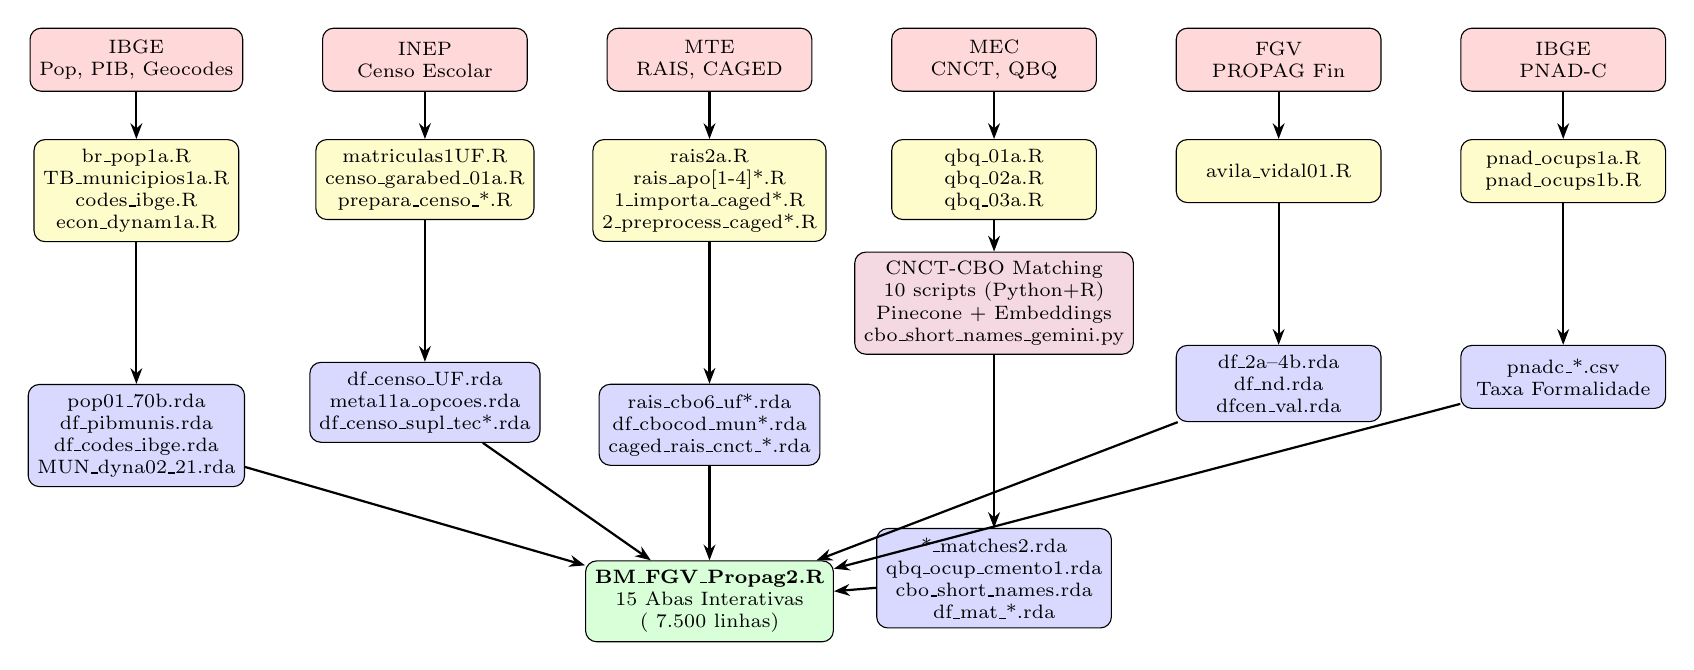
\begin{tikzpicture}[
    node distance=0.6cm and 1.0cm,
    box/.style={rectangle, draw, rounded corners, minimum width=2.6cm, minimum height=0.8cm, align=center, font=\scriptsize},
    rawbox/.style={box, fill=red!15},
    scriptbox/.style={box, fill=yellow!20},
    outputbox/.style={box, fill=blue!15},
    shinybox/.style={box, fill=green!15},
    aibox/.style={box, fill=purple!15},
    arrow/.style={-{Stealth[length=2mm]}, thick}
]

% Row 1: Raw Sources
\node[rawbox] (ibge) {IBGE\\Pop, PIB, Geocodes};
\node[rawbox, right=of ibge] (inep) {INEP\\Censo Escolar};
\node[rawbox, right=of inep] (mte) {MTE\\RAIS, CAGED};
\node[rawbox, right=of mte] (mec) {MEC\\CNCT, QBQ};
\node[rawbox, right=of mec] (fgv) {FGV\\PROPAG Fin};
\node[rawbox, right=of fgv] (pnad) {IBGE\\PNAD-C};

% Row 2: Scripts
\node[scriptbox, below=of ibge] (s1) {br\_pop1a.R\\TB\_municipios1a.R\\codes\_ibge.R\\econ\_dynam1a.R};
\node[scriptbox, below=of inep] (s2) {matriculas1UF.R\\censo\_garabed\_01a.R\\prepara\_censo\_*.R};
\node[scriptbox, below=of mte] (s3) {rais2a.R\\rais\_apo[1-4]*.R\\1\_importa\_caged*.R\\2\_preprocess\_caged*.R};
\node[scriptbox, below=of mec] (s4) {qbq\_01a.R\\qbq\_02a.R\\qbq\_03a.R};
\node[scriptbox, below=of fgv] (s5) {avila\_vidal01.R};
\node[scriptbox, below=of pnad] (s6) {pnad\_ocups1a.R\\pnad\_ocups1b.R};

% Row 2b: AI Pipeline
\node[aibox, below=0.4cm of s4] (ai) {CNCT-CBO Matching\\10 scripts (Python+R)\\Pinecone + Embeddings\\cbo\_short\_names\_gemini.py};

% Row 3: Outputs
\node[outputbox, below=1.8cm of s1] (o1) {pop01\_70b.rda\\df\_pibmunis.rda\\df\_codes\_ibge.rda\\MUN\_dyna02\_21.rda};
\node[outputbox, below=1.8cm of s2] (o2) {df\_censo\_UF.rda\\meta11a\_opcoes.rda\\df\_censo\_supl\_tec*.rda};
\node[outputbox, below=1.8cm of s3] (o3) {rais\_cbo6\_uf*.rda\\df\_cbocod\_mun*.rda\\caged\_rais\_cnct\_*.rda};
\node[outputbox, below=2.2cm of ai] (o4) {*\_matches2.rda\\qbq\_ocup\_cmento1.rda\\cbo\_short\_names.rda\\df\_mat\_*.rda};
\node[outputbox, below=1.8cm of s5] (o5) {df\_2a--4b.rda\\df\_nd.rda\\dfcen\_val.rda};
\node[outputbox, below=1.8cm of s6] (o6) {pnadc\_*.csv\\Taxa Formalidade};

% Row 4: Shiny
\node[shinybox, below=1.2cm of o3] (shiny) {\textbf{BM\_FGV\_Propag2.R}\\15 Abas Interativas\\(~7.500 linhas)};

% Arrows Row 1→2
\draw[arrow] (ibge) -- (s1);
\draw[arrow] (inep) -- (s2);
\draw[arrow] (mte) -- (s3);
\draw[arrow] (mec) -- (s4);
\draw[arrow] (fgv) -- (s5);
\draw[arrow] (pnad) -- (s6);

% Arrows Row 2→3
\draw[arrow] (s1) -- (o1);
\draw[arrow] (s2) -- (o2);
\draw[arrow] (s3) -- (o3);
\draw[arrow] (s4) -- (ai);
\draw[arrow] (ai) -- (o4);
\draw[arrow] (s5) -- (o5);
\draw[arrow] (s6) -- (o6);

% Arrows Row 3→4
\draw[arrow] (o1) -- (shiny);
\draw[arrow] (o2) -- (shiny);
\draw[arrow] (o3) -- (shiny);
\draw[arrow] (o4) -- (shiny);
\draw[arrow] (o5) -- (shiny);
\draw[arrow] (o6) -- (shiny);

\end{tikzpicture}
\end{center}

\newpage

%==============================================================================
% COMPLETE DATA OBJECT LIST
%==============================================================================
\section*{Lista Completa de Objetos de Dados (~40 arquivos .rda + auxiliares)}

\footnotesize
\setlength{\LTleft}{0pt}
\setlength{\tabcolsep}{3pt}
\renewcommand{\arraystretch}{1.3}

\begin{longtable}{p{4.5cm}p{5.5cm}p{4.5cm}p{7cm}}
\toprule
\textbf{Arquivo .rda} & \textbf{Script Criador} & \textbf{S3 Path} & \textbf{Abas que Usam} \\
\midrule
\endfirsthead
\toprule
\textbf{Arquivo .rda} & \textbf{Script Criador} & \textbf{S3 Path} & \textbf{Abas que Usam} \\
\midrule
\endhead
\midrule
\multicolumn{4}{r}{\textit{Continua...}} \\
\endfoot
\bottomrule
\endlastfoot

\multicolumn{4}{l}{\cellcolor{tabA!20}\textbf{DEMOGRAFIA}} \\
pop01\_70b.rda & prelims/população/br\_pop1a.R & working/ibge/ & A1, A2 \\

\multicolumn{4}{l}{\cellcolor{tabA!20}\textbf{CÓDIGOS GEOGRÁFICOS}} \\
df\_codes\_ibge.rda & prelims/mapas/codes\_ibge.R & working/ibge/ & A2, D1, D2, D3, E1 \\

\multicolumn{4}{l}{\cellcolor{tabB!20}\textbf{FINANÇAS PROPAG}} \\
df\_2a.rda \ldots{} df\_4b.rda (8 arquivos) & avila\_vidal01.R & working/fgv/ & B1, B2, B3 \\
df\_nd.rda & avila\_vidal01.R & working/fgv/ & B1, B2, B3 \\
dfcen\_val.rda & avila\_vidal01.R & working/fgv/ & B1, B2, B3 \\

\multicolumn{4}{l}{\cellcolor{tabC!20}\textbf{CENSO ESCOLAR / META 11}} \\
df\_censo\_UF.rda & matriculas1UF.R & working/mec\_inep/ & B1, C1, C2, C3 \\
meta11a\_opcoes.rda & censo\_garabed\_01a.R & working/mec\_inep/ & A2, C1, C2 \\
df\_censo\_supl\_tec23.rda & prepara\_censo\_escolar\_tecnico\_01a.R & working/mec\_inep/ & C3, E1 \\
df\_censo\_supl\_tec24.rda & prepara\_censo\_escolar\_tecnico\_01a.R & working/mec\_inep/ & C3, E1 \\
df\_censo\_notin\_cnct.rda & qbq\_02a.R & working/mec\_inep/ & C3 \\

\multicolumn{4}{l}{\cellcolor{tabC!20}\textbf{PIB E ECONOMIA}} \\
df\_pibmunis.rda & TB\_municipios1a.R & working/ibge/ & C4, D1 \\
df\_residuals\_ols.rda & modelo\_ept3a.R & working/rais/ & C4 \\

\multicolumn{4}{l}{\cellcolor{tabD!20}\textbf{DINAMISMO E APLs}} \\
MUN\_dyna02\_21.rda & econ\_dynam1a.R & working/ibge/ & D1 \\
qbq\_ocup\_cmento1.rda & qbq\_03a.R & working/qbq/ & D2 \\
cbo\_short\_names.rda & qbq\_03a.R + cbo\_short\_names\_gemini.py & working/qbq/ & D2 \\

\multicolumn{4}{l}{\cellcolor{tabD!20}\textbf{INFORMALIDADE}} \\
df\_cbocod\_mun23.rda & rais\_apo4a.R & working/rais/ & D3 \\
df\_cbocod\_mun24.rda & rais\_apo4a.R & working/rais/ & D3 \\

\multicolumn{4}{l}{\cellcolor{tabD!20}\textbf{PNAD-C FORMALIDADE}} \\
pnadc\_*\_uf\_formalidade\_*.csv & pnad\_ocups1a.R / 1b.R & working/pnad/ & D3 \\

\multicolumn{4}{l}{\cellcolor{tabE!20}\textbf{MATCHING OFERTA-DEMANDA}} \\
df\_mat\_uf.rda & qbq\_02a.R & working/mec\_inep/ & E1 \\
df\_mat\_eixo.rda & qbq\_02a.R & working/mec\_inep/ & E1 \\
df\_mat\_area.rda & qbq\_02a.R & working/mec\_inep/ & E1 \\
df\_mat\_curso.rda & qbq\_02a.R & working/mec\_inep/ & E1 \\
df\_exarcu.rda & qbq\_02a.R & working/mec\_inep/ & E1 \\
rais\_cbo6\_uf23.rda & rais2a.R & working/rais/ & E1 \\
rais\_cbo6\_uf24.rda & rais2a.R & working/rais/ & E1 \\
cnct\_qbq\_matches2.rda & qbq\_cnct\_06a.R & working/qbq/ & E1, D2 \\
qbq\_cnct\_matches2.rda & qbq\_cnct\_06a.R & working/qbq/ & E1, D2 \\

\multicolumn{4}{l}{\cellcolor{tabE!20}\textbf{ESCASSEZ PROFISSIONAIS}} \\
caged\_rais\_cnct\_2020\_2024\_shiny.rda & 2\_preprocess\_caged\_rais\_shiny.R & working/mintraemp/ & E2 \\
df\_ranking\_cursos\_caged\_rais.rda & 2\_preprocess\_caged\_rais\_shiny.R & working/mintraemp/ & E2 \\

\end{longtable}

\vspace{1em}
\hrule
\vspace{1em}

\section*{Estrutura do Repositório}

\begin{verbatim}
TechBrazil/
├── RShiny/Produtos2/
│   └── BM_FGV_Propag2.R                # Aplicativo Shiny principal (~7.500 linhas)
│
├── prelims/                             # Scripts de preparação de dados
│   ├── caged/
│   │   ├── 1_importa_caged_rais_cria_df_mun_cbo6.R
│   │   └── 2_preprocess_caged_rais_shiny.R
│   ├── mapas/
│   │   └── codes_ibge.R
│   ├── mec/
│   │   ├── censo_garabed_01a.R
│   │   ├── matriculas1UF.R
│   │   ├── prepara_censo_escolar.R
│   │   └── prepara_censo_escolar_tecnico_01a.R
│   ├── modelo/
│   │   ├── modelo_ept1a.R / 1b.R / 2a.R
│   │   └── modelo_ept3a.R              # Modelo final OLS
│   ├── municipios/
│   │   ├── TB_municipios1a.R
│   │   └── econ_dynam1a.R / 1b.R
│   ├── pnad/
│   │   └── pnad_ocups1a.R / 1b.R
│   ├── população/
│   │   └── br_pop1a.R
│   ├── qbq/                            # QBQ e matching semântico
│   │   ├── qbq_01a.R                   # Importa QBQ bruto
│   │   ├── qbq_02a.R                   # Agrega Censo por curso/eixo
│   │   ├── qbq_03a.R                   # Normaliza ocupações CBO → qbq_ocup_cmento1
│   │   ├── qbq_04a.R                   # Extrai CBOs do CNCT, expande 4-dig → df_cnct_cbo
│   │   ├── cbo_short_names_gemini.py   # Gera nomes curtos CBO via Gemini AI
│   │   ├── cnct1a.py                   # Processa catálogo CNCT
│   │   ├── qbq_cnct1b.py ... 5c.py    # Pipeline matching semântico (8 scripts)
│   │   ├── qbq_cnct5c.R               # Upload S3
│   │   └── qbq_cnct_06a.R             # Enriquecimento final → *_matches2.rda
│   ├── rais/
│   │   ├── rais_download_finaljan10a.R # Download RAIS (versão final)
│   │   ├── rais2a.R                    # Processa vínculos por CBO/UF
│   │   ├── rais3a.R                    # Processa RAIS 2024
│   │   ├── rais_apo1a.R / 1b.R        # APL — cálculo QL
│   │   ├── rais_apo2MUNI.R / 2UF.R    # APL — dados municipais/UF
│   │   ├── rais_apo3MUNI.R / 3UF.R    # APL — matching com cursos
│   │   └── rais_apo4a.R               # Informalidade por município
│   └── avila_vidal/
│       └── avila_vidal01.R             # Simulações financeiras FGV
│
├── docs/
│   ├── relatorio_cnct_cbo_positivo.pdf  # Validação humana matches (confirmar)
│   ├── relatorio_cnct_cbo_negativo.pdf  # Validação humana matches (rejeitar)
│   └── relatorio_cnct_cbo_prova.pdf     # Formulário teste
│
└── working/                             # Dados processados (espelhado no S3)
    ├── ibge/                            # Pop, PIB, geocodes
    ├── mec_inep/                        # Censo Escolar, Meta 11
    ├── fgv/                             # Finanças PROPAG
    ├── qbq/                            # QBQ, matches, cbo_short_names
    ├── rais/                            # Vínculos, APLs, informalidade
    ├── pnad/                            # Formalidade PNAD-C
    └── mintraemp/                       # CAGED/RAIS escassez E2
\end{verbatim}

\end{document}
